\documentclass{article}
\usepackage{xcolor}
\usepackage{amsmath}
\usepackage{amssymb}
\usepackage{amsmath}
\usepackage{amssymb}
\usepackage{pgfplots}
\usepackage{amsmath}
\usepackage{pgfplots}
\usepgfplotslibrary{fillbetween}
\usepgfplotslibrary{groupplots}
\pgfplotsset{compat=1.12}

\begin{document}

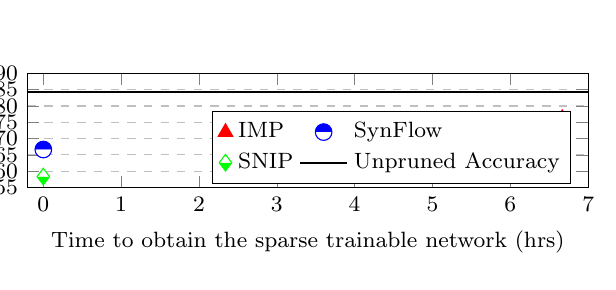
\begin{tikzpicture}[trim axis left,trim axis right,scale=1]
    \begin{axis}[
        width= 8.7 cm,
        height=0.25\textwidth, 
        xlabel={Time to obtain the sparse trainable network (hrs)},
        ylabel={Test accuracy (\%)},
        xmin=-0.2, xmax=7,  % Adjusted the x-axis: 140/36 is approximately 3.89, rounded up to 4 for clarity
        ymin=55, ymax=90,
        xtick={0,1,2,3,4,5,6,7},
        ytick={55,60,65,70,75,80,85,90},
        legend pos=south east,  % Adjusted the legend position
        ymajorgrids=true,
        grid style=dashed,
        legend style={font=\footnotesize, cells={anchor=west}, inner sep=2pt,legend columns=2},  % Adjusted columns
        tick label style={font=\footnotesize},
        label style={font=\footnotesize},
        legend cell align=left,
        mark options={scale=1.5},  % Increase marker size
    ]

    \addplot[
        only marks,
        color=red,
        mark=triangle*,
        ]
        coordinates {
        (24000/3600,76.24)};  % Adjusted the x value
    \addlegendentry{IMP}
        
    \addplot[
    only marks,
    color=blue,
    mark=halfcircle*,
    ]
    coordinates {
    (4.2/3600,66.64)};  % Adjusted the x value
    \addlegendentry{SynFlow}
    
    \addplot[
    only marks,
    color=green,
    mark=halfdiamond*,
    ]
    coordinates {
    (3.13/3600,58.35)};  % Adjusted the x value
    \addlegendentry{SNIP}

    \addplot [mark=none,black,thick] coordinates {
    (-0.5,84.2) (8,84.2)};
    \addlegendentry{Unpruned Accuracy}

    \end{axis}
\end{tikzpicture}

\end{document}